\documentclass[a4paper,11pt]{article}

\usepackage[utf8x]{inputenc}
\usepackage[T1]{fontenc}
\usepackage[french]{babel}
\usepackage{amsmath,amssymb}
\usepackage{fullpage}
\usepackage{xspace}
\usepackage{verbatim}
\usepackage{graphicx}
\usepackage{listings}
\usepackage[usenames,dvipsnames]{color}
\usepackage{url}

\title{Rapport de projet d'algorithmique}
\author{Vivien Matter \and Ernest Foussard}
\date{Avril 2018}

% ===============
\begin{document}
% ===============
\maketitle

\tableofcontents

\newpage

\section{Introduction}

L'objectif du projet était de modifier des graphes de manière à ce qu'il soit
possible d'y trouver un cycle eulerien, puis de le calculer. Pour cela, on a été amenés
à implémenter plusieurs algorithmes et à s'interroger sur la complexité de ces derniers.

\section{Revue des algorithmes}

L'algorithme général se décompose en plusieurs sous-algorithmes: il faut d'abord reconnecter
les composantes connexes du graphe, puis ajouter des arêtes de telle sorte à ce que tous les
sommets soient de degré pairs, et enfin chercher un cycle eulerien.

\subsection{Reconnexion des composantes connexes}

\subsubsection{Algorithme quadratique}

L'algorithme naïf consiste à rechercher toutes les arêtes possibles avec l'ensemble de points
du graphe, de les trier par longueur, puis d'ajouter les segments qui relient deux composantes
connexes distinctes entre elles jusqu'à ce qu'il n'y ait plus qu'une seule composante connexe.
Soit $n$ le nombre de segments du graphe, cet algorithme admet une complexité temporelle $O(n²log(n))$.
On a implémenté une optimisation qui consiste à ne considerer que les arêtes qui relient deux composantes
initialement distinctes, ce qui se réalise facilement avec la structure d'union-find. La complexité dans
le pire des cas (cas où l'ensemble des arêtes est initialement vide) est toujours $O(n²log(n))$, mais
dans les situations pas trop tordues, le gain en temps est considerable.

\subsubsection{Algorithme avec table de hashage}

L'algorithme avec table de hashage consiste à construire un mappage spatial pour repérer les points par rapport
aux autres, et ensuite ajouter de manière gloutonne de manière quasiment ordonnée (on ne trouve pas nécessairement
les plus petits segments, mais les segments du même ordre de grandeur que le plus petit). Le gain en complexité temporelle
est considerable, a priori, et s'écrit $O(nlog(\frac{1}{\alpha}))$ où $\alpha$ est la plus petite distance entre deux points du graphe.
Néanmoins, la complexité spatiale s'écrit $O(4^{\alpha})$ ce qui est extremement problématique dès qu'on a deux points très proches,
car le coût temporel pour instancier de tels objets devient alors très important.
Notre implémentation de cet algorithme ne s'execute pas en temps raisonnable pour la majorité des figures (c'est certainement dû
également à un manque d'optimisation ou une mécomprehension de l'algorithme).
\subsection{Construction du graphe de degrés pairs}

\subsubsection{Algorithme quadratique}

L'algorithme naïf consiste à parcourir l'ensemble des points une première fois pour compter les points de degré impairs,
puis on parcourt l'ensemble des couples de points du graphe par ordre croissant jusqu'à ce qu'il n'y ait plus de sommets de
degré impair, la complexité temporelle de cet algorithme est un $O(n²log(n))$. On a optimisé cet algorithme en ne triant et en n'
iterant que sur les sommets de degré impair. La complexité dans le pire des cas (pavage par des hexagones par exemple : tous les points sont de degré 3) reste un $O(n²log(n))$ mais elle est général bien
moins importante (voir la partie perfomances).

\subsubsection{Algorithme avec table de hashage}

L'itérateur sur les segments ne modifie pas la méthode employée dans l'algorithme précédé, car on
l'applique uniquement sur les points de degré impairs, ce qui conserve l'amélioration faite dans
l'algo précédent. Dans le pire des cas, où on doit parcourir tous les points, la différence entre
cet algorithme et celui quadratique est la même que pour l'algorithme précédent.


\subsection{Détection d'un cycle eulerien}

Pour le calcul d'un cycle eulerien, on a implémenté l'agorithme d'Euler, qui admet une complexité temporelle $O(n)$. Cet algorithme consiste à passer sur des cycles quelconques du graphe en supprimant les segments
utilisés, et pour chaque point de ces cycles refaire cette manipulation. Le fait que le graphe soit à la fois connexe et que toutes
les arêtes soient de degré pairs nous assure la convergence et la correction du code. Comme on ne parcourt qu'une seule fois
chaque arrête du graphe, et que les opérations qu'on effectue lors du parcourt ne sont que des suppressions et des ajouts
de point dans une liste, qui sont instantanées, le passage de l'algorithme est bien en $O(n)$.

\section{Tests de performance}

Du fait qu'ils aient été partiellement optimisés, les algorithmes dépendent plus de la géographie générale des
graphe que du nombre de point.
Pour tester les performances des algorithmes, un programme $tests.py$ a été implémenté, et permet de faire
apparaître le nombre de points et les temps mis par les différents algorithmes pour chaque fichier entré, ces données seront
stoquées dans le fichier $tests_hash.txt$.

\subsection{Reconnect}

Sur une figure déjà connexe, l'algorithme $reconnect$ va être extrêmement performant,
même si elle possède beaucoup de points à traiter, comme on peut le voir sur les deux exemples suivant, respectivement
la figurine 0 et la figurine 20  :
$$ 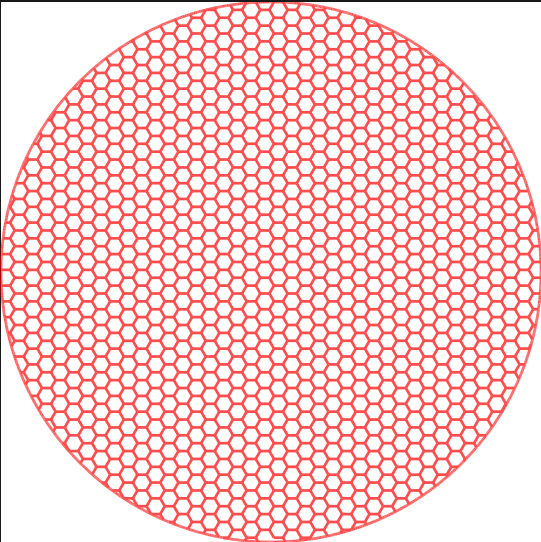
\includegraphics[scale = 0.25]{figurine_0.png} $$
$$ 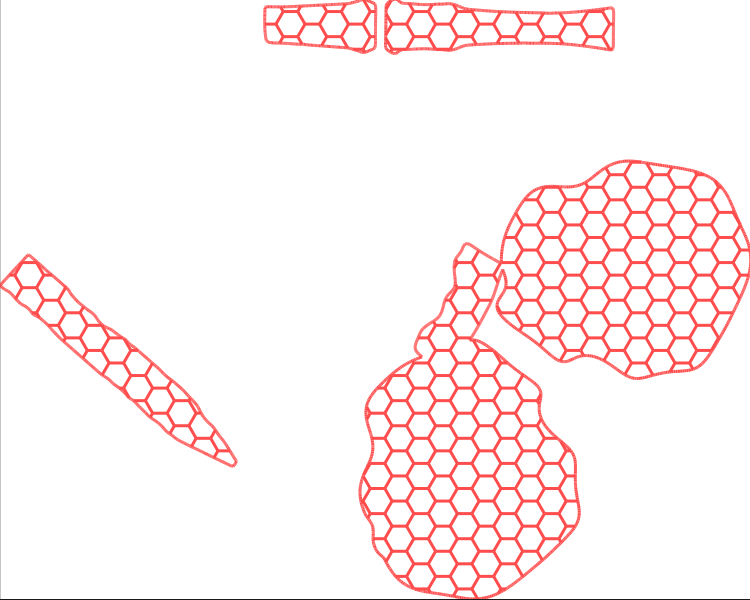
\includegraphics[scale = 0.25]{figurine_20.png} $$
Les deux ont un nombre de segments très similaire : respectivement 5392 et 5362 mais une géométrie très différente :
figurine 0 est déjà connexe, et figure 20 est composée de 3 parties connexes comportants chacune beaucoup de points.
On a ainsi une différence dans le temps d'exécution, où la figurine 0 prend 0.26851797103881836s à être traitée
et la figurine 20 prend 28.114733695983887 s à  être traitée. C'est un rapport supérieur à 100 qui confirme
que les améliorations apportées à l'algorithme $reconnect$ le font fonctionner plus vite, car la version
naïve proposée ne dépend que du nombre de points total et il n'y aurait pas de différence notoire entre ces deux
figure.

\subsection{Even degrees}

De même, la fonction even degrees a été partiellement optimisée en n'itérant que sur les points de degré impair,
ce qui la rend également très dépendante de la géométrie générale des graphes proposés.
Ainsi, en reprenant les deux exemples donnés ci-dessus, on peut encore une fois observer l'utilité de l'optimisation apportée:
La plupart des points de la figure 0 se situent dans des hexagones, et auront donc tous des degrés impairs : on se situe dans le
cas où l'optimisation apportée n'améliore rien car quasiment tous les points sont itérés car de degré impairs.
On effectue ainsi l'algorithme en 30.628416299819946 s.
Dans le cas de la figurine 20, la plupart des points se trouvent dans les bords, où ils n'ont que 2 voisins et sont donc de degré
pairs : l'algorithme n'itère donc que les autres, peu nombreux.
On effectue alors l'algorithme en 2.713702917098999 s, soit plus de 10 fois plus rapidement, et ce cas reste encore loin du cas
optimal où tous les points seraient de degré pair, ce qui donnera à cet algorithme une complexité linéaire.

\subsection{Eulerian cycle}

La fonction eulerian cycle, telle qu'effectue, semble très performante et ne dépend pas de la géométrie de la structure.
Le graphe suivant représente le temps mis par l'algorithme en fonction du nombre de points :
$$ 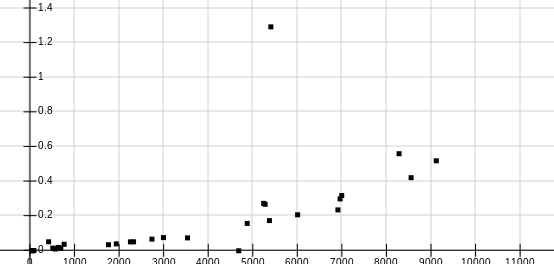
\includegraphics[scale = 0.75]{eularian.png} $$
Il semble ainsi être, conformément à ce qui était prévu, linéaire et indépendant de la géométrie du graphe. (Les points
irréguliers sont dus au passage du ramasse miettes.)
\section{Conclusion}

Les différentes modifications effectuées sur les algorithmes permettent d'avoir un temps d'exécution plus court
qu'avec les algorithmes donnés de base. Nous n'avons pas réussi à faire fonctionner la méthode hash.py suffisement efficacement
pour qu'on arrive à des résultats convenables: il faut néanmoins noter que la méthode quadratique améliorée offre,
une alternative correcte, du moment qu'on ne se situe pas dans le pire des cas. 

\end{document}
